\documentclass[11pt]{report}
\usepackage{titlesec}
\titleformat{\chapter}
{\filcenter\normalfont\Large\bfseries}
{\chaptertitlename~\thechapter} {0.5em} {}

\usepackage[english]{babel}
\usepackage{graphicx}
\usepackage{amsmath,amssymb}
\usepackage{bbm}
\usepackage{listings} %listing R code
\usepackage{siunitx} %voor 10^
\usepackage[usenames,dvipsnames]{color}
\usepackage{color}
\usepackage{enumitem}
\usepackage{pdfpages}
\usepackage{titling}
\usepackage{hyperref}

\setlength{\textheight}{22cm}
\setlength{\topmargin}{-1.5cm}
\setlength{\textwidth}{13cm}
\lstset{frame=shadowbox, rulesepcolor=\color{Gray}, keywordstyle=\color{RoyalBlue}, commentstyle=\color{YellowGreen}, stringstyle=\color{ForestGreen}      % string literal style
} 

\newcommand{\half}{\frac{1}{2}}
\newcommand{\pref}[1]{(\ref{#1})}
\newcommand{\itab}[1]{\hspace{0em}\rlap{#1}}
\newcommand{\tab}[1]{\hspace{.4525\textwidth}\rlap{#1}}

\pretitle{%
  \begin{center}
  \LARGE
  
\includegraphics[width=11.35cm]{logoAAPP}\\[\bigskipamount]
}
\posttitle{\end{center}}

\title{Amsterdam Algorithm Programming Preliminaries Rulebook $2017$}
\author{STORM}
\date{\today}

%%%%%%%%%%%%%%%%%%%%%%%%%%%%%%%%%%

\begin{document}
\selectlanguage{english}
\maketitle
\tableofcontents
\clearpage

\chapter{Definitions}
\begin{description}
\item[AAPP:]
The Amsterdam Algorithm Programming Preliminaries $2017$, also referred to as the contest. The contest is organised by STORM. It will take place on September $23$th, 2017.

\item[BAPC:]
The Benelux Algorithm Programming Contest Finals $2017$ in Amsterdam, organised by study association via (University of Amsterdam). It will take place on October $7$th, $2017$.

\item[NWERC:]
The Northwestern Europe Regional Contest Finale $2017$ at Bath, United Kingdom. It will take place in the weekend of November $24$th, $2017$.

\item[STORM:]
Study association for Mathematics and Computer Sciences studies, at the Vrije Universiteit Amsterdam.

\item[Organisation:]
The members of the organising committee of STORM, also called AAPPCie.

%\item[Website:]
%Maintained by the organisation and among others provides information, problems from previous years and rules Amsterdam Algorithm Programming Preliminaries $2017$. The website is available at \url{http://www.storm.vu/aapp}.

\item[Jury:]
The group of people responsible for checking the solutions submitted by the participants.

\item[Tech:]
The group of people responsible for the system.

\item[Balloon girls:]
Runners who are responsible for delivering print-outs, answering questions and awarding balloons to teams when a submission is correct.

\item[Crew:]
Organisation, members of the jury, tech and balloon girls. 

\item[Participant:]
Member of a participating team that competes in the contest. 

\item[Submission:]
The submission of a solution by a team, which can be handed in using DOMjudge and will be checked by our servers.
\end{description}

\chapter{Organisation}
\begin{enumerate}[label=\bfseries 2.\arabic*]
\item The organisation consists of members of STORM.
\item The organisation has the right to stop the contest, extend the contest time, temporarily block submissions for all teams or change the scores in exceptional conditions.
\item \label{noRules} In situations to which no rule applies, the organisation decides.
\item The jury consists of two jurors to be appointed by the organisation.
\item The organisation has formed the Tech, consisting of students of the Vrije Universiteit Amsterdam.
\item The organisation will appoint balloon girls who will watch over the contest areas during the contest, hand out the print-outs and balloons and will be available for practical questions during the contest.
\item \label{partcipateOrganisation} It is possible for members of the organisation to participate the contest. In that case, the organisation will ensure that this participant will not break section \ref{proofProblemset} and section \ref{proofSolutions}. This means that by section \ref{content}, the chairman of the organisation can not participate in the contest.
\item It is not possible for balloon girls, jury members and tech to participate in the contest, due to the fact that they are helping during the contest.
\item All crew members will be recognizable by their shirt.
\end{enumerate}

\chapter{Participation}
\section{Introduction}
\begin{enumerate}[label=\bfseries 3.1\arabic*]
\item Participation is only possible in student teams of up to $3$ persons, see also section \ref{partcipateOrganisation} if this person is a organisation member.
%\item There are two group stages: one for student teams and one for business teams.
\item Changing the composition of a team is only possible with written permission of the organisation.
\item The organisation decides how many teams are allowed to compete.
\item The organisation has the right to deny the participation of teams before the start of the contest.
\end{enumerate}

\section{Student teams}
A student team:
\begin{enumerate}[label=\bfseries 3.1.\arabic*]
\item may participate for free.
\item consists of students from the Vrije Universiteit Amsterdam and who are not participating in any other team.
%\item has a coach, which is the contact person of a team. This can be a team member or a student or staff member of the institution.
\item participates in the student teams pool for the title 'Winners of the Amsterdam Algorithm Programming Preliminaries $2017$'.
\item \label{BAPC} consists of students who are eligible by the Eligibility Decision Tree (see also appendix), to participate in the student teams pool for a place at BAPC.
\item \label{NWERC} has exactly three students which satisfy section \ref{BAPC}, to participate in the student teams pool for a place at NWERC.
\end{enumerate}

%\section{Business teams}
%A business team:
%\begin{enumerate}[label=\bfseries 3.2.\arabic*]
%\item pays the registration fee of $200$,- euros, before the start of the contest.
%\item consists of persons who are employed by the same company or institution.
%\item participates in the business teams pool for the title 'Winner of the Amsterdam Algorithm Programming Preliminaries $2015$'.
%\end{enumerate}

\chapter{The Contest}
\section{Introduction}
\begin{enumerate}[label=\bfseries 4.1.\arabic*]
\item The language used during the contest is English.
\item The contest lasts for $5$ hours.
\item From the beginning until one hour before the end of the contest, the scores are displayed in DOMjudge.
\item In the last hour, no balloons will be handed out and participants can only see their own score in DOMjudge.
\item The final scoreboard will be shown at the presentation after the contest. %and will be placed on the website.
\item \label{leaveTheWorkplace} If a participant wants to leave the workplace during the contest, for example to use the bathroom or to smoke outside the building, a balloon girl has to accompany him or her.
\end{enumerate}

\section{Problems}
\begin{enumerate}[label=\bfseries 4.2.\arabic*]
\item The jury will provide at least $8$ and at most $12$ problems.
\item When a problem is unclear a 'clarification request' can be sent to the jury. The jury will respond to this request. If the response is relevant to all teams, the jury will send the response to all teams.
\item The jury has the right to change or withdraw problems during the contest. When this happens the jury will inform all teams.
\item \label{content} Before the start of the contest, the content of the problem sets of the AAPP $2017$ and their solutions are known only by the chairman of the organization, the jury and the tech.
\end{enumerate}

\section{Workplace}
\begin{enumerate}[label=\bfseries 4.3.\arabic*]
\item A workplace will be available for each team and all workplaces will be equal in equipment. The following equipment will be provided:
\begin{itemize}
	\item One computer, with two screens, a mouse and a QWERTY keyboard. %see also section \ref{systeminfo} for a specification.
	\item Input data on the computer itself or on the server, see also section \ref{input}.
	\item Paper \& pens.
	\item Three times the problem set of the AAPP $2017$ which can be opened when the contest has started, see also section \ref{Problemset}.
	\item A copy of Rules Amsterdam Algorithm Programming Preliminaries $2017$, including the DOMjudge Team Manual.
\end{itemize}
\item A team is allowed to bring up to $25$ A4-sized pages, printed one-sided or up to $12$ A4- sized pages, printed two-sided, of documentation. Each team member is allowed one identical copy.
\item A team is allowed to bring a dictionary; English to their native language.
\item You may bring mascots such as stuffed toy animals, as long as it does not violate section \ref{hardware}, section \ref{changingHardware} and section \ref{communication}. The mascot needs to be checked before the contest by a crew member.
\end{enumerate}

\section{System}
\begin{enumerate}[label=\bfseries 4.4.\arabic*]
\item A solution has to be written in 
\begin{itemize}
	%\item C
	\item C++
	\item Java
	\item Python
\end{itemize}
unless the problem statement explicitly states otherwise.
%\item \label{systeminfo} The computer we provided runs on Debian and will have the following program(s)/tool(s)/utilitie(s) in alphabetic order:
%\begin{itemize}
%	\item Eclipse
%	\item \ldots
%\end{itemize}
\item \label{input} Input data is provided on your computer. This will be provided once and it will not be uploaded again during the contest.
\item The organisation expects that the teams have read the DOMjudge Team Manual before entering the contest and therefore have the knowledge to be able to hand in a submission, see also appendix for the manual.
\item The jury decides per programming language which libraries and function calls are allowed to be used in the solutions.
\item All prints made by the teams will be brought by a balloon babe. Participants are not allowed near the printers.
\item \label{software}A team is not allowed to bring software.
\end{enumerate}

\section{House rules}
\begin{enumerate}[label=\bfseries 4.5.\arabic*]
\item \label{houserules} The house rules apply to everybody inside the building.
\item \label{hardware} The use of hardware, including all calculators, which are not approved by the organisation are strictly forbidden, with exception of simple watches and medical equipment.
\item \label{mobile} The use of mobile phones, tablets, smart watches or any other electronic device during the contest is strictly forbidden. The organisation will provide safe storage for these devices during the contest.
\item \label{changingHardware} Changing of hardware or operating software is strictly forbidden.
\item \label{communication} During the contest, communication within the team and crew is allowed. Communication with everyone else is forbidden during the contest.
\item \label{crewOrders} Participants must follow any instructions given by the crew.
\item \label{wearTShirt} Participants will wear the shirt and badge provided by the organisation. %(company teams are allowed to wear a shirt with a clear company logo on it).
\end{enumerate}

\section{Judgement}
\begin{enumerate}[label=\bfseries 4.6.\arabic*]
\item Each submission is acknowledged.
\item For each problem, the jury has a correct solution and test data.
\item A submission is correct when it has a solution to the input in a time limit decided by the jury and the output is the same as the output of the jury (unless the problem statement explicitly states otherwise). This time limit is not announced to the teams.
\item The winner of a pool is decided by (in order):
	\begin{enumerate}
	\item The team with the most correctly solved problems.
	\item The team with the least solving time. This is the sum of the time needed for each solved problem (defined as the time between the beginning of the contest and the submission of the first correct solution), plus a $20$-minute penalty for each incorrect submission until the first correct submission. (Incorrect solutions for which a team has not submitted a correct solution or incorrect solutions submitted after a correct solution was accepted do not add to the solving time.)
	\item The team that first submitted its last accepted problem is ranked higher. In case a tie still remains, the team that first submitted its second-last accepted problem is ranked higher, and so on. In the event that this does not resolve the tie, the ranks will be determined by chance.
	\end{enumerate} 
\item The jury is responsible for everything that has to do with the problem set and can be contacted for this through the 'clarification requests'.
\end{enumerate}

\section{Disqualification}
The organisation has the right to disqualify teams for misbehavior/breaking the rules and can use section \ref{noRules} for this. The organisation can disqualify a team among other reasons if the organisation thinks that a participant:
\begin{enumerate}[label=\bfseries 4.7.\arabic*]
\item \label{Problemset} has opened the problem set before the contest started.
\item \label{proofProblemset} had access to the problem set before the contest started.
\item \label{proofSolutions} had access to the solutions before the contest started.
\item does not stick to the House Rules (section \ref{houserules}, section \ref{hardware}, section \ref{mobile}, section \ref{changingHardware}, section \ref{communication}, section\ref{crewOrders} and section \ref{wearTShirt}).
\item did upload software on the computer, against section \ref{software}.
\item did deliberately break section \ref{leaveTheWorkplace}.
\end{enumerate}

\chapter{Prizes}
The organisation and the main sponsor provided the following prize for the participants: %(it is possible to win more than one price as a team)
\begin{enumerate}[label=\bfseries 5.\arabic*]
\item A trophy for the 'Winners of the Amsterdam Algorithm Programming Preliminaries $2017$' including a mechanical keyboard (Cooler Master MasterKeys Pro L White LED Red Switch), for the participants in the student teams pool.
%\item A trophy for the 'Winner of the Amsterdam Algorithm Programming Preliminaries $2015$', for the participants in the business teams pool.
\item A silver medal for the 'Runner-up of the Amsterdam Algorithm Programming Preliminaries $2017$' including a Raspberry Pi $3$ with a case, for the participants in the student teams pool.
\item A bronze medal for the 'Third-place finisher of the Amsterdam Algorithm Programming Preliminaries $2017$' including a powerbank (Trust Urban Primo Powerbank $12.500$ mAh black), for the participants in the student teams pool.
\item At least two places for the BAPC finals, depending on the number of places the organisation of BAPC provides, if the team satisfies section \ref{BAPC}. Transport will be reasonably paid for by the organisation.
\item At least two places for the NWERC depending on the number of places the organisation of NWERC provides, if the team satisfies section \ref{NWERC}. NWERC teams are selected by the scores on BAPC. Transport and accommodation will be reasonably paid for by the organisation, up to a certain amount. 
\end{enumerate}

\chapter{Appendix}
See next pages for the
\begin{itemize}
\item Eligibility Decision Tree
\item Domjudge Team Manual including a NWERC scoreboard example
\end{itemize}
\clearpage

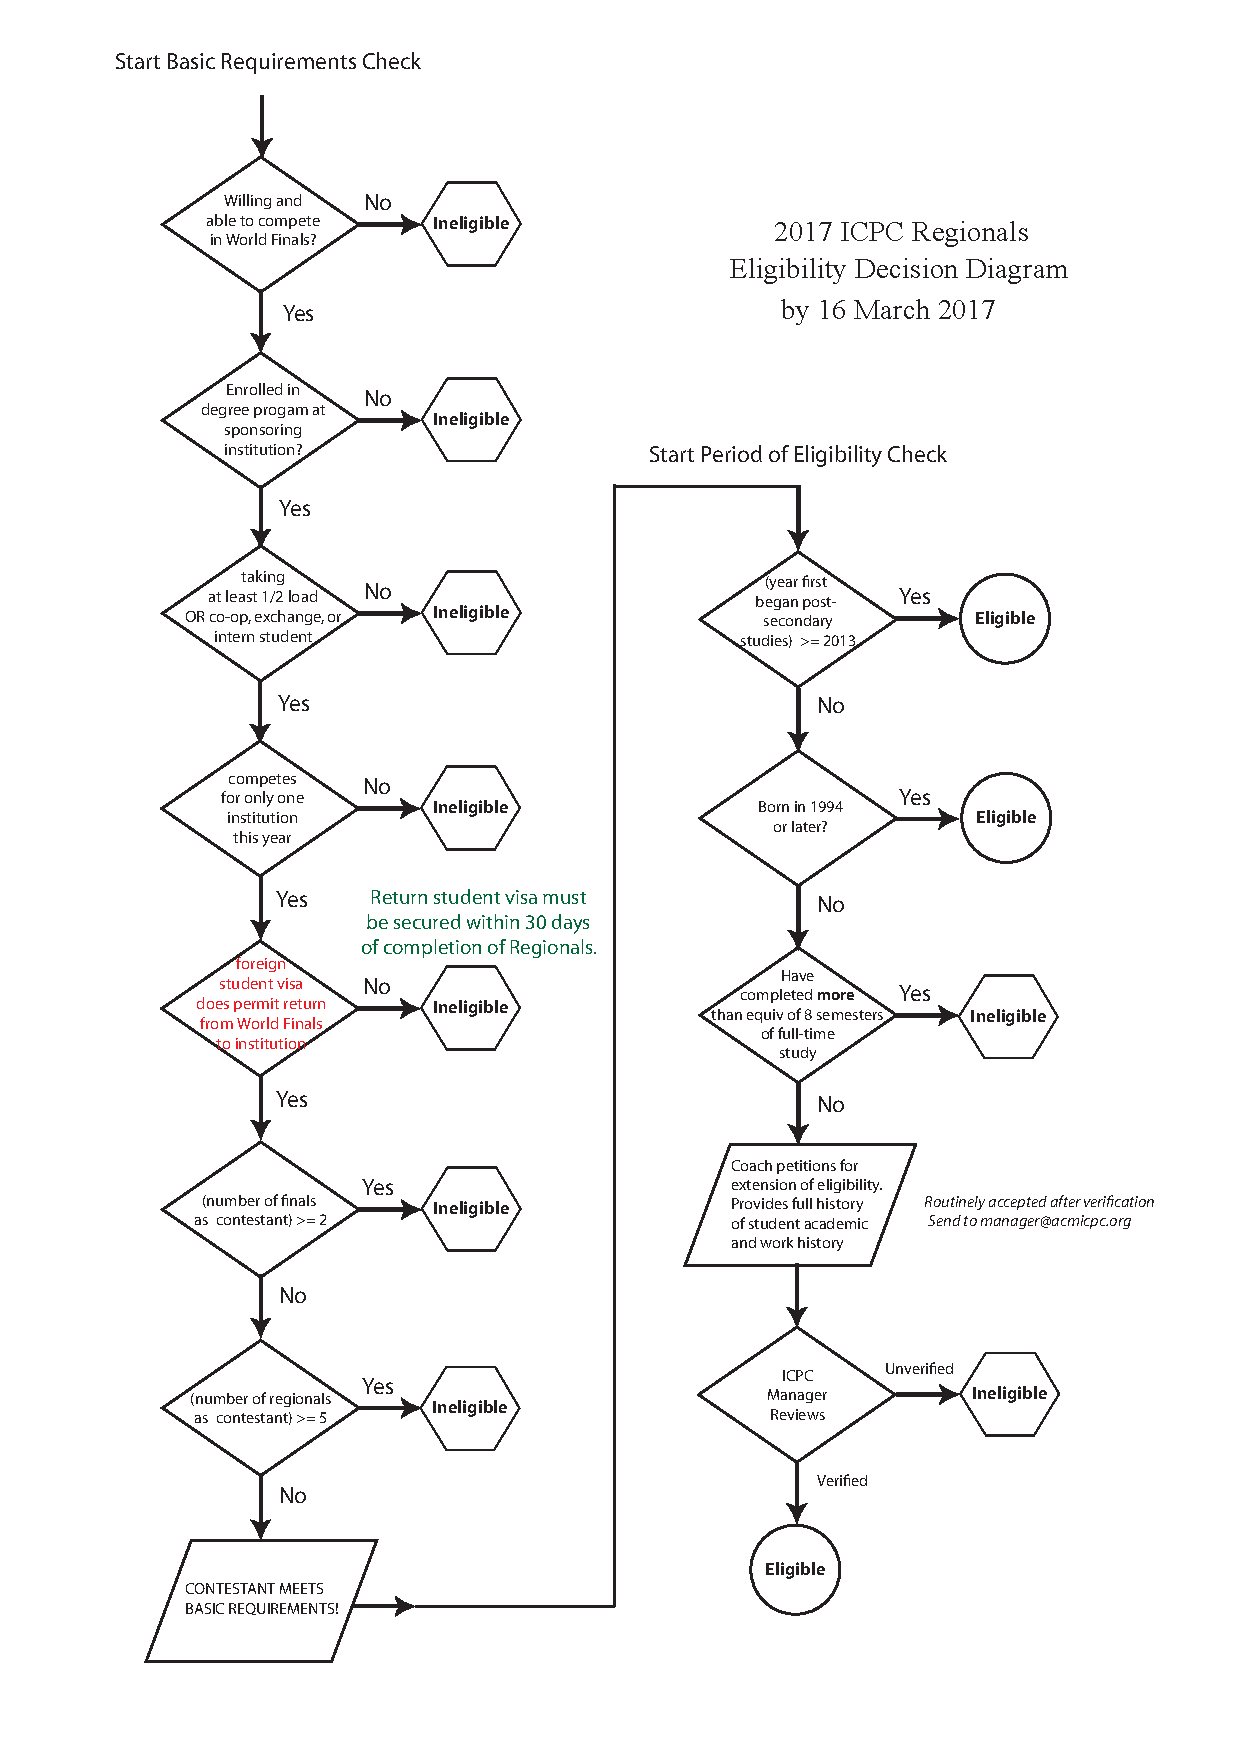
\includepdf[pages={1}]{EligibilityDecisionTree-2017.pdf}
\addcontentsline{toc}{subsection}{Eligibility Decision Tree}

\begin{center}
\vspace*{\fill}
This page is intentionally left blank.
\vspace*{\fill}
\end{center}
\clearpage

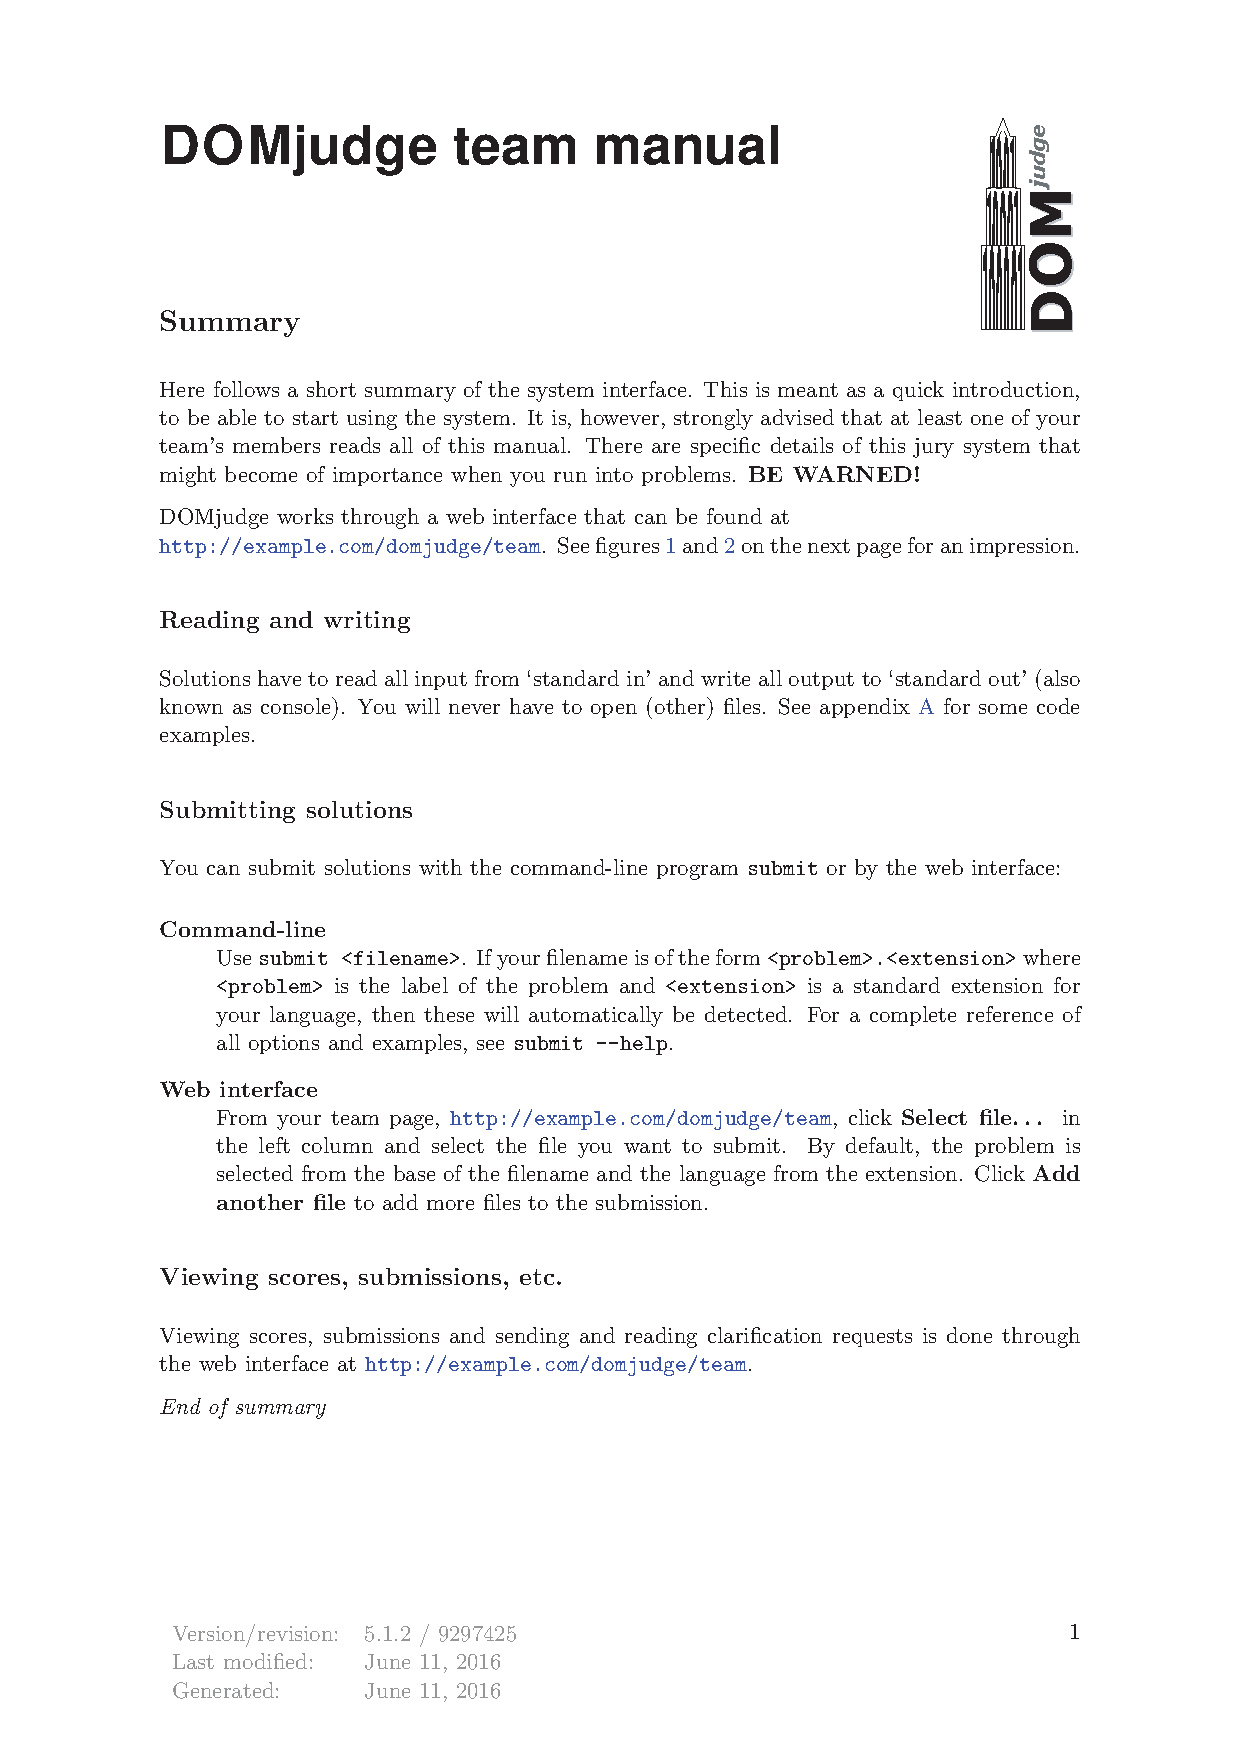
\includepdf[pages={1-9}]{team-manual.pdf}
\addcontentsline{toc}{subsection}{DOMjudge team manual, including a NWERC scoreboard example}

\end{document}